{\bf BME154L - Spring 2012 - Exam \#2 Solutions}\hfill Name (Net ID):\underline{\hspace*{3.0in}}



\section{[30 points]}

Various physiologic systems in the body can be represented as second-order
systems.  Below is a voltage trace from a lab group measuring the output
(impulse response) of the system you designed in Lab 8 with a finger tap
(``delta-like'') input.

\begin{figure}[htb!]
\centering
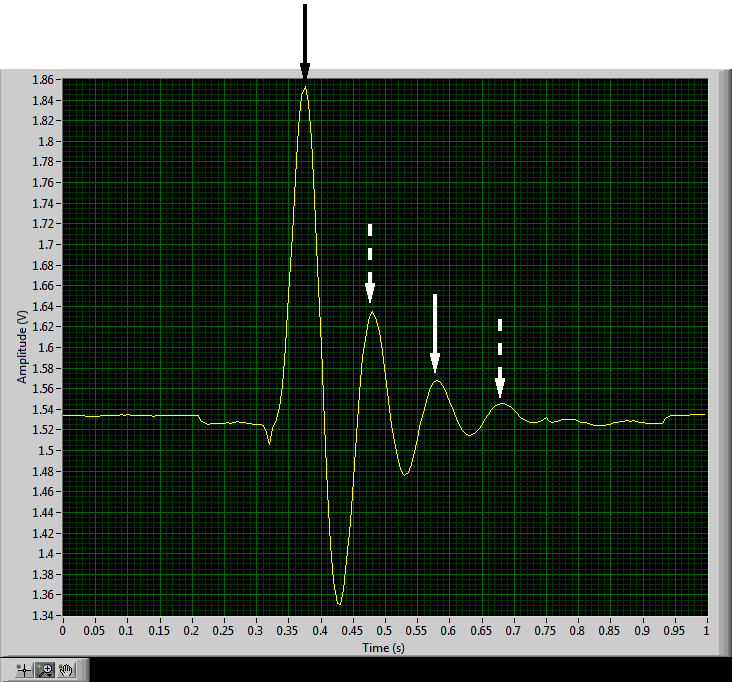
\includegraphics[width=0.5\linewidth]{impresp.png}
\caption{Second-Order System Impulse Response}
\label{fig:impresp}
\end{figure}

\begin{enumerate}

\item The oscillations in Figure~\ref{fig:impresp} occur at the damped
frequency of this system ($\omega_d$).  Is $\omega_d$ greater than or less than
the natural frequency ($\omega_n$) of this system given this impulse response?
Why? [5 points]

\item Bandwidth:
\begin{itemize}
    \item What is the relative bandwidth (greater or less) of this impulse
response compared to that of a continuous sinusoid oscillating at $\omega_d$?
Why? [5 points]
    \item What would happen to the bandwidth of this impulse (increase or decrease) if the damping coefficient of this system increased?  Why?  [5 points]
\end{itemize}

\item Draw the block diagram for a circuit that powers an LED with a 0.7 V
threshold voltage on every {\bf other} positive peak of the impulse response
signal above 1.54 V (two solid arrows in Figure~\ref{fig:impresp}) (i.e., use
the impulse response as the input signal into your circuit).  The LED can
remain on until the next temporal positive peak occurs (dashed arrows in
Figure~\ref{fig:impresp}).  Be as detailed as possible in your block diagram.
[15 points]

\end{enumerate}

\clearpage

{\bf BME154L - Spring 2012 - Exam \#2 Solutions}\hfill Name (Net ID):\underline{\hspace*{3.0in}}



\clearpage

{\bf BME154L - Spring 2012 - Exam \#2 Solutions}\hfill Name (Net ID):\underline{\hspace*{3.0in}}



\clearpage

{\bf BME154L - Spring 2012 - Exam \#2 Solutions}\hfill Name (Net ID):\underline{\hspace*{3.0in}}



\clearpage

